\documentclass{article}

\usepackage[usenames,dvipsnames]{color}
\usepackage{graphicx}
\usepackage{bytefield}
\usepackage{hyperref}
\usepackage{listings}

\definecolor{lightgray}{gray}{0.8}
\definecolor{lightblue}{rgb}{0.92,0.92,1.0}
\definecolor{lightred}{rgb}{1.0,0.92,0.92}

\newcommand{\rcolor}{lightblue}
\newcommand{\wcolor}{lightred}
\newcommand{\reserved}{lightgray}

\newenvironment{packed_itemize}{
\begin{itemize}
  \setlength{\itemsep}{1pt}
  \setlength{\parskip}{0pt}
  \setlength{\parsep}{0pt}
}{\end{itemize}}

\newenvironment{packed_enum}{
\begin{enumerate}
  \setlength{\itemsep}{1pt}
  \setlength{\parskip}{0pt}
  \setlength{\parsep}{0pt}
}{\end{enumerate}}

\hypersetup{
    bookmarks=true,         % show bookmarks bar?
    unicode=false,          % non-Latin characters in Acrobat’s bookmarks
    pdftoolbar=true,        % show Acrobat’s toolbar?
    pdfmenubar=true,        % show Acrobat’s menu?
    pdffitwindow=false,     % window fit to page when opened
    pdfstartview={FitH},    % fits the width of the page to the window
    pdftitle={My title},    % title
    pdfauthor={Author},     % author
    pdfsubject={Subject},   % subject of the document
    pdfcreator={Creator},   % creator of the document
    pdfproducer={Producer}, % producer of the document
    pdfkeywords={keyword1} {key2} {key3}, % list of keywords
    pdfnewwindow=true,      % links in new window
    colorlinks=true,        % false: boxed links; true: colored links
    linkcolor=black,        % color of internal links
    citecolor=green,        % color of links to bibliography
    filecolor=magenta,      % color of file links
    urlcolor=cyan           % color of external links
}

\lstset{ %
language=C,                     % the language of the code
basicstyle=\footnotesize,       % the size of the fonts that are used for the code
numbers=none,                   % where to put the line-numbers
numberstyle=\footnotesize,      % the size of the fonts that are used for the line-numbers
stepnumber=2,                   % the step between two line-numbers. If it's 1, each line 
                                % will be numbered
numbersep=5pt,                  % how far the line-numbers are from the code
backgroundcolor=\color{white},  % choose the background color. You must add \usepackage{color}
showspaces=false,               % show spaces adding particular underscores
showstringspaces=false,         % underline spaces within strings
showtabs=false,                 % show tabs within strings adding particular underscores
frame=single,                   % adds a frame around the code
tabsize=2,                      % sets default tabsize to 2 spaces
captionpos=b,                   % sets the caption-position to bottom
breaklines=true,                % sets automatic line breaking
breakatwhitespace=false,        % sets if automatic breaks should only happen at whitespace
title=\lstname,                 % show the filename of files included with \lstinputlisting;
                                % also try caption instead of title
escapeinside={\%*}{*)},         % if you want to add a comment within your code
morekeywords={*,...}            % if you want to add more keywords to the set
}

\newcommand{\colorbitbox}[4][lrtb]{%
  \bitbox{0}{}%
  \rlap{\bitbox[#1]{#3}{\color{#2}\rule{\width}{\height}}}%
  \bitbox[#1]{#3}{#4}}
\newcommand{\colorwordbox}[4][lrtb]{%
  \bitbox{0}{}%
  \rlap{\wordbox[#1]{#3}{\color{#2}\rule{\width}{\height}}}%
  \wordbox[#1]{#3}{#4}}

\begin{document}

\begin{abstract}
Peanuts are tasty.
\end{abstract}

\section{Overview}

Programmable hardware is increasingly deployed in large, physically distributed control systems.
Hard real-time systems especially benefit from the determinism and low latency of purpose-built hardware.
As reconfigurable hardware components replace traditional software-based systems, 
those hardware components must often communicate directly, over longer distances.
While traditional protocols like CORBA and SOAP 
provide an excellent abstraction for software-to-software communication,
they are a poor fit for hardware-to-hardware communication.
Hardware components typically transfer information in read/write bus cycles
as opposed to the procedure calling interfaces seen in software.

The Etherbone protocol takes an existing bus standard (Wishbone~\cite{wishbone}) 
and extends this bus to run over the network.
A concrete bus standard was chosen, 
because different bus protocols often differ enough that conversion reduces fidelity.
Wishbone was chosen because it is an open standard, simple, and pipe\-lining.
The underlying transport protocol is left open,
as Etherbone's require\-ments are easily met.
This specification defines Etherbone for UDP and TCP.

Etherbone's key features are:
\begin{packed_itemize}
\item Bus-cycle interface
\item Deterministic latency
\item Simple hardware implementation
\item Cut-through/wormhole operation
\item Compatible with software implementations
\item Separate config/control address space
\item Negotiable bus/address widths
\end{packed_itemize}

Etherbone leaves these issues to the lower transport layer:
\begin{packed_itemize}
\item Exactly once delivery (TCP or reliable layer 2)
\item Cut-through switching
\item Authentication (physical access or TLS)
\item Confidentiality
\end{packed_itemize}

%Etherbone was built for use by the GSI/FAIR and CERN/LHC particle accelerator projects.
%Thus, it is used in control systems which span approximately 2 and 20 kilometres respectively.
%As a companion to the WhiteRabbit project~\cite{white-rabbit}, it runs over Gigabit ethernet.
%Assuming fiber optics, the flight times are 10$\mu$s and 100$\mu$s,
%while buffering a 1500-byte Ethernet frame takes 12$\mu$s.

Etherbone was designed for the following use cases:
\begin{packed_itemize}
\item High-precision system control
\item Sensor data acquisition
\item System diagnostics
\item Remote debugging
\item Distributed bus bridging
\end{packed_itemize}

%\section{Related Work}

% RMAP spacewire ESA
%  specific transport
%  unspecified bus protocol
% RDMA for large transfers in HPC (infiband, ethernet and tcp/ip)

\section{Architecture}

Etherbone (EB) connects two Wishbone (WB) buses together as shown in
Figure~\ref{fig:hw-system}.
The WB Intercon is a local bus, for example a crossbar interconnect.
When a WB master wishes to write to a remote slave, 
it writes to the EB bridge,
which is a local WB slave.
The bridge, acting as an EB master, 
translates the request into an EB frame
(Section~\ref{sec:packet-format}) and routes it to
the receiving EB slave.
That slave decodes the request and executes the write over Wishbone.
Finally, the WB interconnect routes the write to the correct slave.

\begin{figure}[t]
\centering%
\includegraphics[width=\columnwidth]{system}
\caption{Etherbone system in hardware}
\label{fig:hw-system}
\end{figure}

Either or both of the devices in Figure~\ref{fig:hw-system} may be replaced by software,
as shown in Figure~\ref{fig:sw-system}.
In this scenario,
the operating system buffers and sends Etherbone frames as requested by the
Etherbone software library.
Client applications may use this library for remote access to
any slave attached to an Etherbone equipped wishbone bus.
This facilitates such tasks as debugging, firmware updates, and monitoring from a
dekstop system.
Applications may also attach devices to a virtual wishbone bus,
perhaps to capture bus cycles or trigger an alarm.
These virtual devices may be mapped into the Wishbone bus of other Etherbone nodes,
hardware or software.

\begin{figure}[t]
\centering%
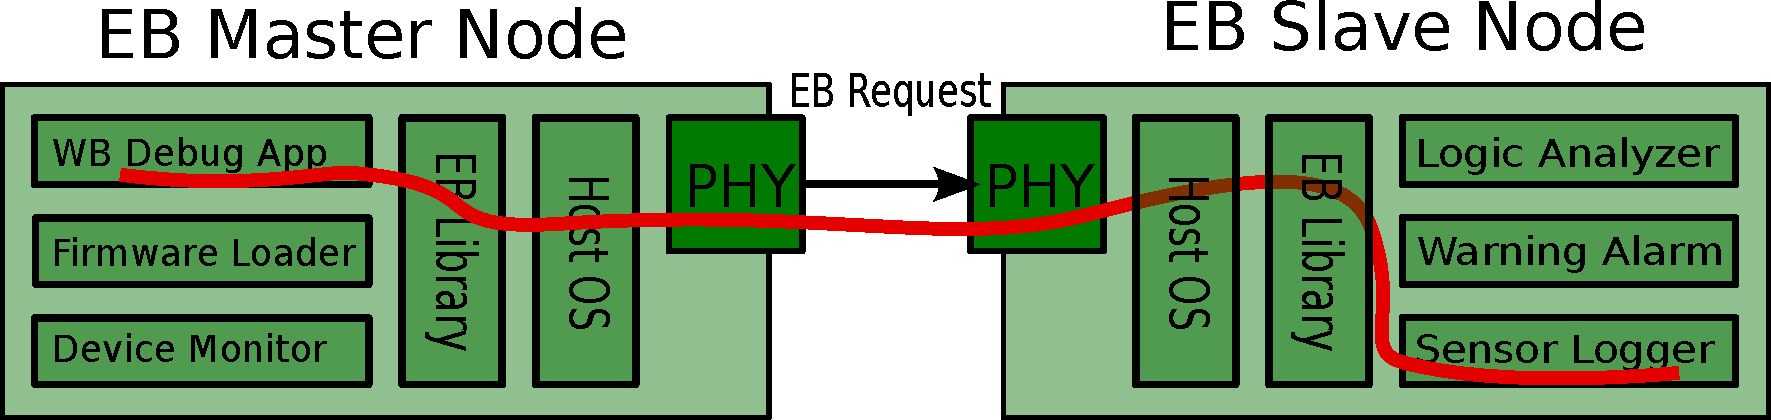
\includegraphics[width=\columnwidth]{software}
\caption{Etherbone system in software}
\label{fig:sw-system}
\end{figure}

\subsection{Addressing}

Slaves on a Wishbone bus have a mapped address range.
Masters read and write to an address on the local bus
and the Intercon routes the operation to the matching slave device.
However, with the introduction of Etherbone, 
there are now multiple reachable Wishbone buses in the facility-wide system.
To select the destination slave, additional address information is required.

When using the software interface,
an application acquires a handle object for the remote bus.
Reads and writes are then performed via the handle object,
requiring only the WB bus address per operation.
To acquire the handle object, 
the application supplies the hostname and port of the remote WB bus.

For a hardware implementation,
the requests come from a local WB master,
which can only provide a WB bus address.
%The WB protocol provides no As the WB pro Requests cannot carry any additional address information to select the WB bus.
To determine the missing address information,
an EB bridge must infer the destination WB bus 
based only on the local WB address requested.
To achieve this,
the EB bridge establishes a configurable mapping from local WB addresses to
destination hostname:ports and target WB addresses.

For example, 
consider an EB bridge occupying address range 0x1000-0x3000 on the local bus.
There is a remote WB bus available on the the host example.com:3434.
We would like to access the address range 0x100-0x200 on that bus.
Thus, we configure our EB bridge to map this range as 0x2000-0x2100 on the
local bus.
Now, when a WB write on our local bus to address 0x2050 is performed,
the bridge transforms this into an EB write destined for example.com:3434 
at address 0x150.

\subsection{Pipelining}
\label{sec:pipeline}

Unlike a local WB bus, where devices answer in a few clock cycles,
a remote bus accessed via EB has a much high latency.
For a 100MHz bus and a distance of only 20km the difference is
10ns to 100$\mu$s. 
For Internet-scale distances, the latency can easily rise to 100ms.
Therefore, 
an application which only issues a new read/write operation when the previous
operation completes will perform $10^4$ to $10^7$ times slower over EB than direct WB.

EB supports pipelining to overcome this significant performance bottleneck.
Instead of issuing a single operation at a time,
an application/device can issue new operations without waiting
for the previous operation to complete.
The results of the operations will arrive in the same order they were issued.
Whenever new operations do not dependend on still incomplete operations,
this can almost entirely mask the performance lost to remote access.

As an example, considering two application using EB.
The first application is a firmware writing tool that needs to write the
firmware and confirm the firmware was written correctly.
This problem can be readily pipelined; 
the operations have an order requirement (confirmation happens after write),
but the choice of operation to issue does not depend on previous results.
The firmware writer can issue a sequence of WWWW...RRRR... operations
in the pipeline without waiting.
Alternatively, it might also use the sequence WRWRWR... to confirm each word
immediately after writing it.
In both cases, the application can issue all of the operations without waiting.
This would not be possible if the application were to iterate a remote function.
Suppose the application wants to compute $f(f(f(...f(x)...)))$ 
using a remote WB slave to calculate function $f$.
Here, the aplication writes $x$ to the remote slave and reads back
$y = f(x)$.
Then the application writes $y$ to the remote slave and reads back
$z = f(y)$.
The write pattern WRWRWR... is the same as the firmware loader,
but here we can only pipeline a single write-read operation pair together.
Until we have received the result $f(x)$, we cannot issue $f(y)$.

In Wishbone, several operations can be grouped into a single bus cycle.
A particularly bad situation that can occur is when dependencies appear within a WB cycle.
Generally, WB cycles acquire the device for use until cycle completion.
On a local bus, any access pattern will work, 
as the operations will complete quickly and release the cycle line.
However, when this happens with EB-sized latencies, 
a cycle might tie up a device for potentially unacceptable duration.
Consider for example a WB cycle that reads from one address 
and writes the result to another address.
Locally, there is no problem; the entire WB cycles executes in a few
nanoseconds.
However, when that same access pattern runs over the network,
the slave device needs to wait for the read result to travel to the master and the final write to travel back.
A very bad design.

Dealing with data dependencies within a cycle is a major complication
addressed in the different implementation options described in
Section~\ref{sec:eb-master}.

\subsection{Config Space}

In addition to remote bus access, 
Etherbone also provides a configuration space.
This config space is used to specify transmission parameters,
recover bus error status codes,
and match read results to the requests.

The config space is an complementary 16-bit wide address space attached to every EB slave.
EB requests can read/write to this configuration space in addition the the normal WB bus.
The config space is divided up into two regions: the register space and the implementation space.
All addresses in the register space correspond to EB control registers,
specified in this document.
The register space spans addresses 0x0-0x7FFF.
The implementation space is guaranteed to be free for whatever use
a hardware/software implementation chooses.
The implementation space spans 0x8000-0xFFFF.

Two important registers in the address space include the error status
register, which reports WB error status codes, and the WB device map pointer,
which provides information about the slaves attached to a remote bus.
The implementation space is typically used by an EB master to receive
the data which it read.
Reads to an EB device trigger a write back to the source EB device.
Those writebacks are often sent to the implementation space 
where they can be handled by the EB core/code and invisible to the WB bus.

\subsection{Bus Widths}

In Wishbone, 
a bus may have a port width that is 8/16/32/64 bits wide.
Thus, a master in one WB bus might write 32-bits at a time,
while a slave in another WB bus expects 16-bits at a time.
Etherbone makes no attempt to convert between differing port widths,
because converting a 32-bit write into two 16-bit writes might change semantics.

However, 
Etherbone does negotiate which port widths are acceptable to both devices.
This mostly affects software,
which can meaningfully support access with different port widths.
Hardware implementations will typically advertise and accept only one width.

Address spaces in WB are conceptually infinite, 
but in practice are constrained to a fixed width.
Address width conversion, as oppposed to port width conversion,
is relatively straight-forward.
Address 0x0400 is that same as 0x00000400.
If a 32-bit device is accessed by a 16-bit device,
the 16-bit device can only see the low 16-bits of the larger device's address space.

Address width is negotiated by Etherbone simply to determine the amount of
space to reserve for message exchanges.
A hardware implementation is free to only advertise address widths
whose message alignment is convenient to them.

\section{Real-time Deployment}
\label{sec:deployment}

One of the key features of Etherbone is that it can used with hard realtime constraints
and extremely low latency.
In this scenario, Etherbone only forms a small part of the complete system.
To meet deadlines, presumably most components must make timing guarantees.
The Etherbone software library, 
due to its dependency on the host operating system,
cannot guarantee responsiveness.
Therefore, in a hard real-time system,
the software library can be used neither as slave nor master.

Beyond those timing requirements imposed externally, 
Etherbone requires attached slave devices to respond quickly.
As detailed in Section~\ref{sec:cut},
Etherbone slaves can use cut-through request processing to avoid buffering delays.
In this situation, 

\subsection{Multimaster competition}

\subsection{Master-Slave cross-talk}
%... master gets his answer in
%... but he is also a slave and gets traffic there too
%=> must have physically distinct cables 

\subsection{Cut-Through}

\section{Programmer Guide}

Etherbone is designed to transport the Wishbone bus over the network.
In the Wishbone bus, every participant is either a master or a slave.
Only masters may issue requests and only slaves may service them.

A request is either a read or a write and includes the target address.
If the request is a write, it also includes the word to store.
A response includes a success/failure status bit and (if a read) the word read.

Etherbone is pipelined.
A master may issue multiple requests without waiting for a response.
These requests are transmitted in ordered batches called a cycle.
This pipelined behaviour is essential for high throughput over a network.
%With a typical 125MHz wishbone bus, requests can be issued every 8ns.
%Over the network, the round trip latency may exceed 200$\mu$s.

An application may use Etherbone to implement either a bus master or slave.
For both scenarios there is a hardware and software interface.

\subsection{Software Interface}

\begin{figure}[t!]
\centering
\begin{tabular}{|l|p{0.7\textwidth}|}
\hline
Type & Purpose \\
\hline
eb\_status\_t &
An error status result from an Etherbone API call.
Can be converted to text with eb\_status().
Takes values from Table~\ref{fig:status}.
\\
eb\_socket\_t & 
Top-level object handle used in the Etherbone library. 
An application must first create a socket to use any other library feature.
\\
eb\_flags\_t &
Options which control the type of eb\_socket\_t created.
\\
eb\_width\_t &
A bitmask which lists acceptable Wishbone bit widths.
8/16/32/64 are the possible alternatives.
\\
eb\_descriptor\_t &
An operating system specific socket handle.
This can be extracted from an eb\_socket\_t to use with operating system event handling.
\\
eb\_address\_t & 
A 64-bit wide unsigned integer type for Wishbone addresses.
If the software application only advertises a 16-bit address bus,
the unused high bits are required to be zero.
\\
eb\_data\_t & 
A 64-bit wide unsigned integer type for Wishbone data.
If the negotiated bus port width is less than this,
the unused high bits are required to be zero.
\\
eb\_cycle\_t & 
A collection of queued Wishbone read/write operations.
Operations are executed in order with the target device held busy for the
cycle duration.
Operations will not begin execution until the cycle is closed.
\\
eb\_device\_t &
A handle to a remote Wishbone bus.
Used to open a new eb\_cycle\_t.
\\
eb\_network\_address\_t &
A hostname:port string used to identify a remote Etherbone bridge.
\\
eb\_handler\_t &
A virtual Wishbone device.
These may be attached to an eb\_socket\_t and accessed remotely.
\\
eb\_user\_data\_t &
An opaque pointer type.
Whenever an Etherbone library permits a user callback function,
a eb\_user\_data\_t may be supplied that is provided to the callback upon
completion.
This is useful to record state associated with the operation needed upon
completion.
\\
\hline
\end{tabular}
\caption{Etherbone software library type definitions}
\label{fig:types}
\end{figure}

\begin{figure}
\centering
\begin{tabular}{|l|p{0.6\textwidth}|}
\hline
Status Code & Purpose \\
\hline
EB\_OK & 
The operation completed successfully. 
\\
EB\_FAIL & 
The operating system reported an error.
\\
EB\_ADDRESS & 
Invalid address; 
too large for the negotiated bus.
\\
EB\_WIDTH & 
Invalid data; 
too large for the negotiated bus.
\\
EB\_OVERFLOW & 
Cycle length was too long for the chosen protocol.
This only applies to UDP transport.
\\
EB\_BUSY & 
The object cannot be closed as it is in use by derived objects.
\\
\hline
\end{tabular}
\caption{Etherbone result status codes}
\label{fig:status}
\end{figure}

The Etherbone software library relies on the host operating system to
implement TCP and UDP.
Therefore,
strict timing requirements cannot be assured and 
maximum throughput will be somewhat below the physical limit.
Nevertheless, 
this interface to Etherbone is useful since the 
application can leverage a higher-level development enviroment.

\subsubsection{Etherbone Sockets}

All interaction with the Etherbone library begins with opening an Etherbone socket
using \texttt{eb\_socket\_open}.
The socket is used to send and receive Etherbone messages over TCP or UDP.
In order for the library to process incoming messages, 
the socket must be regularly polled by the application.
Be aware that the Etherbone library is not thread-safe.
All access to a socket and any derived objects must be from a single-thread.
Different threads may make use of distinct sockets safely, however.

There are three approaches a software Etherbone application can take to
managing activity on the Etherbone socket:
\begin{packed_enum}
\item 
Watch the Etherbone socket for activity in an external event loop,
for example, a GUI's top-level main loop. 
To support this, the method \texttt{eb\_socket\_descriptor} allows access to the
underlying operating system socket descriptor.
The external framework can then watch this for readability,
and call \texttt{eb\_socket\_poll} to process the pending messages.
\item
Regularly call \texttt{eb\_socket\_poll} while doing calculations.
This frees the application to fully utilize the CPU for calculations,
but still handles Etherbone messages.
The responsiveness and performance of Etherbone in this scenario will depend
on how frequently \texttt{eb\_socket\_poll} is called. 
Every 1-4ms is a good target.
If there are no calculations to perform, 
this approach wastes a lot of CPU time needlessly testing the socket.
\item
Use \texttt{eb\_socket\_block} to halt the application until messages arrive.
Then, run \texttt{eb\_socket\_poll} to process the events.
Repeat until Etherbone is no longer of interest to the application.
As opposed to polling, 
this lets the CPU idle when there is no pending traffic.
\end{packed_enum}

Figure~\ref{fig:socketm} lists the prototypes of the relevant methods. 
See Figure~\ref{fig:types} for an explanation of the types,
and Figure~\ref{fig:status} for the potential return codes.
The socket may be either TCP or UDP as controlled by the mutually exclusive
eb\_flags\_t options EB\_UDP\_MODE and EB\_TCP\_MODE. 
A valid port width argument is the bitwise OR of EB\_DATA\{8,16,32,64\},
or EB\_DATAX for all of them.
Similarly, EB\_ADDR\{8,16,32,64,X\} defines the acceptable address widths.
The header files provide detailed pre- and post-conditions for using the methods.

\begin{figure}
\centering
\begin{lstlisting}
eb_status_t eb_socket_open(
    int           port, 
    eb_flags_t    flags,
    eb_width_t    supported_addr_widths,
    eb_width_t    supported_port_widths,
    eb_socket_t*  result);

eb_status_t     eb_socket_close     (eb_socket_t socket);
eb_status_t     eb_socket_poll      (eb_socket_t socket); 
int             eb_socket_block     (eb_socket_t socket, 
                                     int timeout_us);
eb_descriptor_t eb_socket_descriptor(eb_socket_t socket);
\end{lstlisting}
\caption{Etherbone socket control methods}
\label{fig:socketm}
\end{figure}

\subsubsection{Master Mode}

An Etherbone application can become a master on a remote Wishbone bus.
To begin this mode of operation, 
the application first opens the remote bus with \texttt{eb\_device\_open}.
This initiates negotiation of the bus address and data widths,
resulting in a wire format to be used for Etherbone cycles.
The relevant methods appear in Figure~\ref{fig:devicem}.

Thereafter, the Etherbone application creates bus cycles.
Each cycle performs a sequence of read or write operations
\footnote{For UDP sockets,
only 150 operations may be queued per cycle.}.
Until the cycle is closed, it is not queued to be sent.
Thus, data dependencies (Section~\ref{sec:pipeline}) within a cycle
are prevented,
greatly improving the responsiveness of Etherbone.

Because network protocols perform most efficiently with larger transfers,
the Etherbone library delays transmission of a cycle until
either the local buffer is full or the the buffer is flushed with
\texttt{eb\_device\_flush}.
The methods involved are listed in Figure~\ref{fig:cyclem},

Putting this all together,
to write to a remote register an Etherbone application needs to take these
steps:
\begin{packed_enum}
\item Open an Etherbone socket (\texttt{eb\_socket\_open})
\item Open an remote device's bus (\texttt{eb\_device\_open})
\item Begin a new Wishbone cycle (\texttt{eb\_cycle\_open})
\item Enqueue a write operation (\texttt{eb\_cycle\_write})
\item Mark the end of the cycle (\texttt{eb\_cycle\_close})
\item Flush the buffers out the socket (\texttt{eb\_device\_flush})
\item Close the device and socket or begin a new cycle.
\end{packed_enum}

After a cycle has been executed remotely, 
the application-supplied callback will be invoked 
indicating that the reads have completed and 
providing error status for each operation.

Due to the packet format of Etherbone (Section~\ref{sec:fmt}),
be aware that writing sequentially is more bandwidth efficient than random
access.

\begin{figure}
\centering
\begin{lstlisting}
eb_status_t eb_device_open(
    eb_socket_t           socket, 
    eb_network_address_t  ip_port, 
    int                   attempts,
    eb_device_t*          result);

eb_status_t eb_device_close        (eb_device_t device);
eb_socket_t eb_device_socket       (eb_device_t device);
eb_width_t  eb_device_port_width   (eb_device_t device);
eb_width_t  eb_device_address_width(eb_device_t device);   
\end{lstlisting}
\caption{Etherbone remote bus access methods}
\label{fig:devicem}
\end{figure}

\begin{figure}
\centering
\begin{lstlisting}
typedef void (*eb_cycle_callback_t)
   (eb_user_data_t, eb_status_t, eb_bool_t*);

eb_cycle_t eb_cycle_open_read(
    eb_device_t          device,
    eb_user_data_t       user,  
    eb_cycle_callback_t  cb);

void eb_cycle_close(eb_cycle_t cycle);
void eb_cycle_read (eb_cycle_t, eb_address_t, eb_data_t* data);
void eb_cycle_write(eb_cycle_t, eb_address_t, eb_data_t  data);

void eb_device_flush(eb_device_t socket);
\end{lstlisting}
\caption{Etherbone remote cycle methods}
\label{fig:cyclem}
\end{figure}

\subsubsection{Slave Mode}

An Etherbone application can register virtual devices on a simulated Wishbone bus.
These devices may then be remotely accessed by Etherbone masters.
There is one virtual bus per Etherbone socket.
The EB address is the application system's hostname and the
port provided on socket creation.

For maximum interoperability, 
software slave devices should support access at any data width;
this is not much of a burden when compared with hardware.
Slaves on a socket must all share the same supported address and port widths, 
as they are all on the same virtual Wishbone bus.
 
A virtual device claims a base address and mask,
in the virtual socket bus.
This address range must not overlap 
any other virtual slave devices attached to this socket.
Address decoding and bus arbitration are handled by the library internally.

Each virtual device provides a read and write callback,
as shown in Figure~\ref{fig:vdevm}.
These callbacks must return immediately and may not generate a bus error.
Accesses to unmapped virtual addresses will always produce a bus error.

\begin{figure}
\centering
\begin{lstlisting}
typedef struct eb_handler {
  eb_address_t base;
  eb_address_t mask;
  
  eb_user_data_t data;

  /* Values for Wishbone device autodiscovery */
  uint16 wbd_version;
  uint32_t vendor;
  uint32_t device;
  uint32_t wbd_flags;
  uint32_t hdl_class;
  uint32_t hdl_version;
  uint32_t hdl_date; /* e.g: 0x20111225 -- christmas 2011 */

  eb_data_t (*read) (eb_user_data_t, eb_address_t, eb_width_t);
  void      (*write)(eb_user_data_t, eb_address_t, eb_width_t, 
                     eb_data_t);
} *eb_handler_t;

eb_status_t eb_socket_attach(eb_socket_t, eb_handler_t handler); 
eb_status_t eb_socket_detach(eb_socket_t, eb_address_t address);
\end{lstlisting}
\caption{Etherbone virtual device methods}
\label{fig:vdevm}
\end{figure}


\subsection{Hardware}

\begin{figure}[t]
\centering%
\includegraphics[width=\columnwidth]{etherbone_internals}
\caption{Etherbone hardware}
\label{fig:hw-impl}
\end{figure}

To be written by Matthias.

\section{Protocol and Implementation}

This section details the Etherbone protocol.
All conformant devices must adhere to the message format outlined in
Section~\ref{sec:fmt}.
Optional design considerations are explicitly indicated in the text.
Every other behaviour described in this section is mandatory for a
conforming Etherbone hardware or software implementation.

\subsection{Message Format}
\label{sec:fmt}

%\begin{figure}[t!]
% \centering
 \settowidth{\bitwidth}{\scriptsize BCAi}
 \begin{bytefield}{16}
  \bitheader{0,4,7,8,16} \\
  \bitbox{16}{\nameref{field:Magic} (0x4E6F)}  \\
  \bitbox{4}{\nameref{field:Version}} &
  \colorbitbox{\reserved}{3}{} &
  \bitbox{1}{\rotatebox{90}{\small \nameref{field:PF}}} &
  \bitbox{4}{\nameref{field:AddrSz}} &
  \bitbox{4}{\nameref{field:PortSz}} \\
  \wordbox{2}{Potential padding to 64-bit alignment} \\
  \wordgroupl{\rotatebox{90}{EB Record (Repeats)}}
   \bitbox{1}{\scriptsize \nameref{field:RCA}}&
   \bitbox{1}{\scriptsize \nameref{field:BCA}}&
   \bitbox{1}{\scriptsize \nameref{field:RFF}}&
   \colorbitbox{\reserved}{1}{} &
   \bitbox{1}{\scriptsize \nameref{field:CYC}}&
   \bitbox{1}{\scriptsize \nameref{field:WCA}}&
   \bitbox{1}{\scriptsize \nameref{field:WFF}}&
   \colorbitbox{\reserved}{1}{} &
   \bitbox{4}{\nameref{field:RCount}} &
   \bitbox{4}{\nameref{field:WCount}} \\
   \wordbox{1}{Potential padding to 32-bit alignment} \\
   \wordbox{2}{Potential padding to 64-bit alignment} \\
   \wordgroupr{\rotatebox{270}{\nameref{field:RCount} $\not= 0$}}
    \colorwordbox{\rcolor}{1}{\nameref{field:BaseRetAddr}} \\
    \colorwordbox{\rcolor}{1}{\nameref{field:ReadAddr} 1} \\
    \colorwordbox{\rcolor}{1}{\nameref{field:ReadAddr} 2} \\
    \colorwordbox[tb]{\rcolor}{1}{$\vdots$ \\[1ex]} \\
    \colorwordbox{\rcolor}{1}{\nameref{field:ReadAddr} $N$}
   \endwordgroupr \\
   \wordgroupr{\rotatebox{270}{WCount $\not= 0$}}
    \colorwordbox{\wcolor}{1}{\nameref{field:BaseWriteAddr}} \\
    \colorwordbox{\wcolor}{1}{\nameref{field:WriteVal} 1} \\
    \colorwordbox{\wcolor}{1}{\nameref{field:WriteVal} 2} \\
    \colorwordbox[tb]{\wcolor}{1}{$\vdots$ \\[1ex]} \\
    \colorwordbox{\wcolor}{1}{\nameref{field:WriteVal} $N$}
   \endwordgroupr
  \endwordgroupl \\
 \end{bytefield}
% \caption{Etherbone Message Format}
% \label{fig:header}
%\end{figure}

\subsubsection{Etherbone Header}

An Etherbone message contains an Etherbone header followed by a 
sequence of records.
Records are processed in the order they appear in the message.

All reserved fields (indicated in grey) must be cleared to 0.
All numeric values have bigendian format.
Packet alignment is max(16, \nameref{field:AddrSz}, \nameref{field:PortSz}).
For Etherbone version 1, this is either 16, 32 or 64 bits.

The Etherbone header immediately follows the encapsulating UDP or TCP header.
If the packet alignment exceeds 32-bits, 
the header is followed by zeros padding to the alignment size.

\paragraph{Magic} \label{field:Magic}

As Etherbone is layered atop UDP or TCP, 
stray messages might find their way to Etherbone endpoints.
In order to indentify the Etherbone protocol,
every valid Etherbone message includes the value 0x4E6F as a prefix.
Any packet missing this magic protocol identifier must be dropped.

\paragraph{Version} \label{field:Version}

This document describes Etherbone version 1.

Future Etherbone revisions must retain support for obsolete
Etherbone messages formats.
Etherbone responses must use the same version as the request
which triggered the response.

If an Etherbone device receives a request for an unsupported version,
it should ignore the request unless \nameref{field:PF} is set.
When \nameref{field:PF} is set, the largest of the requested version
and the supported version should be returned.

\paragraph{PF} \label{field:PF}

The Probe-Flag (PF) is used to negotiate compatible bus width and version.
In a message with PF set,
the highest Etherbone version supported appears in \nameref{field:Version}.
Furthermore, a probe message must be 64-bit aligned, so the 32-bit pad is mandatory.
The contents of \nameref{field:AddrSz} and \nameref{field:PortSz} will be ignored.

Upon receipt of a message with PF set, 
an Etherbone device should ignore the remainder of the message
and respond with an Etherbone header with the PF field cleared.
The supported address and data bus widths of the Etherbone
device should appear in the \nameref{field:AddrSz} and \nameref{field:PortSz} fields.
The \nameref{field:Version} field should contain the largest of the
requested version and the supported version.

\paragraph{AddrSz} \label{field:AddrSz}

In principle, 
Wishbone buses do not have a fixed address width.
The value AddrSz specifies the number of bits used 
to represent addresses in Etherbone messages.
Only the low address bits are included,
any necessary higher bits should be considered zero.

The values for AddrSz are listed below.
They may be added together to indicate support for multiple widths.
When an Etherbone message contains multiple AddrSz values
or the receiving device does not support the selected value, 
any content beyond the header is ignored.

\vspace{1em}
\begin{tabular}{|l|l|}
\hline
AddrSz & Address bits \\
\hline
1 & 8 \\
2 & 16 \\
4 & 32 \\
8 & 64 \\
\hline
\end{tabular}

\paragraph{PortSz} \label{field:PortSz}
The Wishbone standard permits interconnection of slaves and masters 
with bus data widths of 8/16/32/64.
Masters must use the correct data bus width when communicating with slaves.
PortSz specifies the data bus width of the target slave.

The values for PortSz are listed below.
They may be added together to indicate support for multiple widths.
When an Etherbone message contains multiple PortSz values
or the receiving device does not support the selected value, 
any content beyond the header is ignored.

\vspace{1em}
\begin{tabular}{|l|l|}
\hline
PortSz & Data bus width \\
\hline
0 & 8 \\
2 & 16 \\
4 & 32 \\
8 & 64 \\
\hline
\end{tabular}

\subsubsection{Record Header}

Each record in an Etherbone stream includes a header.
If the packet alignment exceeds 16-bits, 
the header is followed by zeros padding to the alignment size.

\paragraph{RCA} \label{field:RCA}
If the addresses read in this record should be taken from the config
address space, the RCA flag is set.
Otherwise values will be read from the Wishbone bus.

\paragraph{BCA} \label{field:BCA}
If the BaseRetAddr is in the config space of the originating EB device,
the BCA flag is set.
The value of this flag is copied to the matching WCA field.

\paragraph{RFF} \label{field:RFF}
If the results of Wishbone reads should be written back to a FIFO register
located at BaseRetAddr, the RF flag is set.
Otherwise read values will be written sequentially starting at the
BaseRetAddr.

\paragraph{CYC} \label{field:CYC}
If the contents of this record are the last of a cycle,
the CYC flag is set.
A receiving EB device should hold the cycle line high till it encounters this flag.

\paragraph{WCA} \label{field:WCA}
If the values written in this record should be written to a the config
address space, the WCA flag is set.
Otherwise values will be written to the Wishbone bus.

\paragraph{WFF} \label{field:WFF}
If the values written in this record should be written to a FIFO register,
the WF flag is set.
Otherwise values will be written sequentially starting at BaseWriteAddr.

\paragraph{RCount} \label{field:RCount}
This Wishbone record includes RCount reads.
The message will include an equal number of \nameref{field:ReadAddr} fields.

\paragraph{WCount} \label{field:WCount}
This Wishbone record includes WCount writes.
The message will include an equal number of \nameref{field:WriteVal} fields.

\subsubsection{Read Data Section}

Read fields are processed in order.

\paragraph{BaseRetAddr} \label{field:BaseRetAddr}
This field is present only if \nameref{field:RCount} $>$ 0.
If the \nameref{field:AddrSz} is shorter than the packet alignment, 
the address is big-endian zero extended.
When it exists it indicates the address on the origin Etherbone endpoint 
to which read results should written.

\paragraph{ReadAddr} \label{field:ReadAddr}
For each ReadAddr, 
a read operation to that address will be executed.
Depending on the value of \nameref{field:RCA},
the address is either a config space or Wishbone bus read.
If the \nameref{field:AddrSz} is shorter than the packet alignment, 
the address is big-endian zero extended.
Results are written back to \nameref{field:BaseRetAddr} on the origin endpoint.

\subsubsection{Write Data Section}

Write fields are processed in order.

\paragraph{BaseWriteAddr} \label{field:BaseWriteAddr}
This field is present only if \nameref{field:WCount} $>$ 0.
If the \nameref{field:AddrSz} is shorter than the packet alignment, 
the address is big-endian zero extended.
When it exists it indicates the address on the target Etherbone endpoint 
to which values should written.
If \nameref{field:WCA} is set,
writes go to the config space,
otherwise the address is on the Wishbone bus.

\paragraph{WriteVal} \label{field:WriteVal}
For each WriteVal, 
a write operation will be executed.
If the \nameref{field:PortSz} is shorter than the packet alignment, 
the value is big-endian zero extended.
The destination address is computed from \nameref{field:BaseWriteAddr} and 
\nameref{field:WFF}.


\subsection{Config Registers}
\label{sec:config}

Config registers are always 64-bits wide.
If \nameref{field:PortSz} less than 64-bit is supported,
a EB slave device must support sub-word access.
For example, an 8-bit read to address 7 must return the
low 8-bits of register 0.
EB master device access to config registers must always be aligned.
A 32-bit read to address 2 has undefined result.

So far, there are only two config registers defined:

\begin{tabular}{|l|p{0.7\textwidth}|}
\hline
Register & Purpose \\
\hline
0 &
Error status.
This shift register records the error status for completed Wishbone
operations.
If the last operation was successful,
the low bit of this register is zero.
Therefore, 
after an Etherbone master issues a cycle containing 13 operations,
it can read this register to determine the error status using the low
13-bits of the register.
\\
\hline
8 &
Address of the Wishbone autodiscovery header.
Every Etherbone device must include somewhere in its config address space
a Wishbone autodiscovery structure.
This structure describes all devices attached to the local Wishbone bus.
\\
\hline
\end{tabular}

\subsection{UDP and TCP streams}

The Etherbone protocol is embedded directly in both UDP and TCP.
In both cases, the protocol format and handling remains the same.
The Etherbone protocol is designed to be processed as a stream;
for UDP datagrams that stream is simply packed into a single message.
For TCP, the stream consumes the entire TCP connection,
probably split into many TCP/IP segments over the wire.

With UDP operation,
each message includes a fresh Etherbone header.
The packet contents can be considered as a (short) Etherbone stream
whose format adheres to Section~\ref{sec:fmt}.
A master should end the cycle by setting CYC in the last record.
By design,
an Etherbone response can never be longer than the Etherbone request
which triggered it.
Therefore, whenever a UDP/IP request arrives, 
the UDP response will fit in the same sized IP frame.
Etherbone does not add reliability to UDP.
If reliable operation over UDP is required, 
link layer FEC should be used.

For TCP operation,
the entire TCP stream appears like a single Etherbone stream;
there is only one Etherbone header at the very beginning of the stream.
To probe a device requires an initial short-lived TCP connection,
since everything after the header is ignored.
TCP adds reliability and congestion control to Etherbone,
but at the cost of determinism.
Because TCP retransmits lost segments in order,
a single loss will stall all following operations,
a phenomenon known as head-of-line blocking.
TCP Etherbone hardware device is also quite expensive to implement.

For real-time reliable hardware, UDP is the appropriate choice.
It is faster, deterministic, and cheaper in FPGA area.
Whenever software requires access over an unreliable link,
like the global Internet,
TCP access is the better choice.
One solution to this mismatch is to put an Etherbone TCP-UDP gateway
at the edge of the reliable internal network.
This (software) bridge can also implement access control,
requiring TCP Etherbone connections to run over ssh port forwarding.

\subsection{Server / Slave Operation}

The Etherbone format was carefully designed to make it stream process.
It is possible to process an incoming UDP datagram and
begin sending an outgoing response 
without either the incoming or outgoing Ethernet frame ever touching a buffer.
This approach is described in Section~\ref{sec:cut}.

\subsubsection{Header processing}

Any stream with invalid \nameref{field:Magic} is ignored in its entirety.
Otherwise the \nameref{field:Magic} is copied to the outgoing stream.

If the \nameref{field:PF} flag is set,
the response stream includes the maximum of the locally supported
\nameref{field:Version} and the \nameref{field:Version} included in the request.
The response also lists all supported \nameref{field:AddrSz} and \nameref{field:PortSz}.
The rest of the incoming stream is ignored,
and the output stream is aligned to 64-bits then terminated.

If the \nameref{field:AddrSz} or \nameref{field:PortSz} include multiple entries, 
the remainder of the stream is ignored.

\subsubsection{Record processing}

A response record header is created from a request record header by the
following transformation:
\begin{packed_itemize}
\item 0 $\to$ \nameref{field:RCA}
\item 0 $\to$ \nameref{field:BCA}
\item 0 $\to$ \nameref{field:RFF}
\item \nameref{field:CYC} $\to$ \nameref{field:CYC}
\item \nameref{field:BCA} $\to$ \nameref{field:WCA}
\item \nameref{field:RFF} $\to$ \nameref{field:WFF}
\item 0 $\to$ \nameref{field:RCount}
\item \nameref{field:RCount} $\to$ \nameref{field:WCount}
\end{packed_itemize}

If \nameref{field:RCount} is non-zero,
the \nameref{field:BaseRetAddr} is copied from the input stream to the
output stream where it will fill the \nameref{field:BaseWriteAddr} slot.
Each \nameref{field:ReadAddr} is then read from either the config space or
Wishbone bus according to the \nameref{field:RCA} flag.
The results are written to the output stream.

If \nameref{field:WCount} is non-zero,
the \nameref{field:BaseRetAddr} is stored to a variable $x$.
For each \nameref{field:WriteVal}, 
a write is issued to address $x$ on either the Wishbone bus or config space
depending on the \nameref{field:WCA} flag.
If \nameref{field:WFF} is set, 
$x$ is incremented by \nameref{field:PortSz} after each operation.

While processing writes,
an Etherbone slave has two options for the output stream.
It can either write nothing, saving bandwidth,
or it can write \nameref{WCount}+1 zeros.
The advantage to filling in zeros is that it makes the outgoing stream exactly
the same length as the incoming stream.

After completion of each read or write operation,
the EB slave shifts the error status into config register 0
(Section~\ref{sec:config}).
This can be read by the EB master to determine the error status of the
operation.

\subsubsection{Cut-through}
\label{sec:cut}

To achieve extremely low latency,
a hardware Etherbone slave can operate in cut-through mode.
Here, 
each read/write operation is pipelined to the Wishbone bus.
As the Wishbone acknowledgements arrive,
the outgoing stream is filled in normally.

In order to stream an outgoing UDP frame,
the slave must implement a buffer large enough to fit an IP+UDP header.
Once the slave has determined that it will answer a request
(after processing the Etherbone header),
it fills the IP+UDP headers with fields appropriate 
to respond to the origin device.
The UDP checksum is set to 0 as the UDP payload is not available for
checksum in time for cut-through mode;
this is allowed by RFC 768.
The outgoing IP length is set to the same as the incoming length;
this is why Etherbone supports zero padding for write operations.

Streaming out this initial UDP+IP header buys the local bus some 
latency for responding to requests.
However, the local Wishbone bus must process requests faster than the
physical connection Etherbone uses to send.
Otherwise, the out-going Etherbone stream would starve and create a 
corrupt packet.
Real-time implementations must, therefore, 
ensure every slave on their Wishbone bus has sufficient bandwidth.

One wrinkle that must be dealt with is Wishbone cycle termination.
There are three problems: 
stalling between cycles, 
status register stalls,
incomplete cycles.
They will be discussed in turn.

Unfortunately, a Wishbone cycle cannot end until all the acknowledgements
have completed.
Therefore,
before processing the next cycle in the stream,
the Etherbone slave must stall until the previous cycle completes.
Each such stall slowly eats into the latency margin 
won by the IP+UDP header.
The only way to ensure these stalls do not starve the response stream
is to guarantee that every operation is acknowledged within the time
it takes to stream three words minus two cycles.
Since the record header and address can be queued in one cycle each,
every record wins two words of latency minus two cycles.
Since every cycle includes at least one record and one operation,
this means the bus can always keep up with transmission if
the pipeline depth does not exceed three words delay.
To make this concrete,
suppose the Wishbone bus is 32-bit wide 125MHz and 
the output is Gigabit ethernet.
Now, every attached Wishbone slave must 
guarantee acknowledgement within 10 cycles
(3*32*125MHz/1GHz-2).

The next problem is that the error status register depends on Wishbone
error status codes.
Those codes only arrive with the operation completion.
Thus, whenever a record reads the config space,
the EB slave must stall until all outstanding Etherbone operations complete.
Fortunately, the same restriction needed for cycle termination stalls
is sufficient to also cover this case.
Every transition from Wishbone bus access to config space access costs
at least two words for the new record header.

Finally, there is the sticky issue about how to handle 
a stream that never ends the cycle.
There are two options:
honour this request or ignore it.
If the device chooses to honour the request,
it will block the local Wishbone bus until the next stream arrives.
If it does not honour the requset,
an operation that should have been atomic might be broken.
Notice that
a software Etherbone master / client will never issue a request of this form.
Unfortunately, 
transparent bridging (Section~\ref{sec:bridge}) always generates requests like this.
Ultimately, 
further operations continuing a cycle from a previous stream
is a pathological case caused by a poorly designed WB master
with an in-cycle data dependency (Section~\ref{sec:pipeline}).
The chosen behaviour is left open as an implementation decision,
but it is probably wisest to implicitly terminate cycles on stream end.

\subsection{Client / Master Operation}
\label{sec:eb-master}

An Etherbone master issues requests to remote Wishbone buses.
It might be a software client,
a hardware EB client,
or a bridge device that maps a remote bus locally.
In any case, the task is fairly straight-forward:
transform read/write operations into Etherbone messages.

One important design consideration is how to handle read results.
The config space reserves the range 0x8000-0xFFFF for implementation use.
Probably the best implementation approach is to use this space as the
\nameref{field:BaseRetAddr} in read requests.
The resulting write-back can then be matched to the triggering read.

\subsubsection{Software Client}

A software client is by far the simplest.
A small internal table records the 
callback information needed for each outstanding cycle.
The \nameref{field:BaseRetAddr} is used as an index into this table.

Read/write operations are enqueued on a per cycle basis.
Once the cycle is closed,
the library looks to see if the writes can be compressed into a FIFO or
sequential write stream.
Otherwise it just streams the operations out as a sequence of records.
Every 64 operations, 
it injects a config register read to recover error status codes.

\subsubsection{Hardware Client}

A hardware client is not much more sophisticated than a software client.
We assume that this client is generating the requests itself,
not translating them from a local bus.

Presumably, 
it's requests have a regular format 
and it doesn't even need the sophistication of 
a software client's pattern matching for FIFO/sequential access.

For demanding real-time applications,
a dedicated hardware Etherbone master is the best approach.
Bridging can achieve similar latency,
but only a hardware client can fully utilize available bandwidth.

\subsubsection{Bridge Mode}
\label{sec:bridge}

Unfortunately, 
a Wishbone cycle cannot end until all the acknowledgements are received.
The Etherbone bridge cannot issue acknowledgements until 
it receives Etherbone responses.
Thus, Wishbone cycles cannot complete faster than a network round-trip.
This completely kills the throughput of bridged bus.
Despite the poor throughput, 
reasonable latency can still be attained.

Keeping this in mind,
we can safely assume that any high performance Etherbone master will use 
a dedicated hardware client and not be built on a bridge.
Many sticky implementation issues below can be resolved by 
trading bandwidth for simplicity.
Given the inherent limitations to bridging,
this seems a reasonable trade-off.

A bridge should start streaming out a fixed length UDP/IP Etherbone 
request as soon as a Wishbone cycle begins.
Without buffering,
an unknown access pattern cannot be compressed.
Therefore, 
a bridge simply translates each operation into a separate Etherbone record.
Whenever there is no pending operation,
the bridge just writes zeros (an empty Etherbone record).
If operations come faster than space is available in the stream,
stall the Wishbone master until space is available.
When the currently streamed message runs out of space,
stall the master until the response has arrived.
As most Wishbone cycles are short,
this is a pragmatic way to avoid the huge buffers needed to 
fixup reponse message mis-ordering.

\end{document}

